\tikzstyle{level 1}=[level distance=5cm, sibling distance=2cm]
\tikzstyle{level 2}=[level distance=5cm, sibling distance=1cm]
\tikzstyle{bag} = [text width=4em, text centered]
\tikzstyle{end} = [circle, minimum width=3pt,fill, inner sep=0pt]
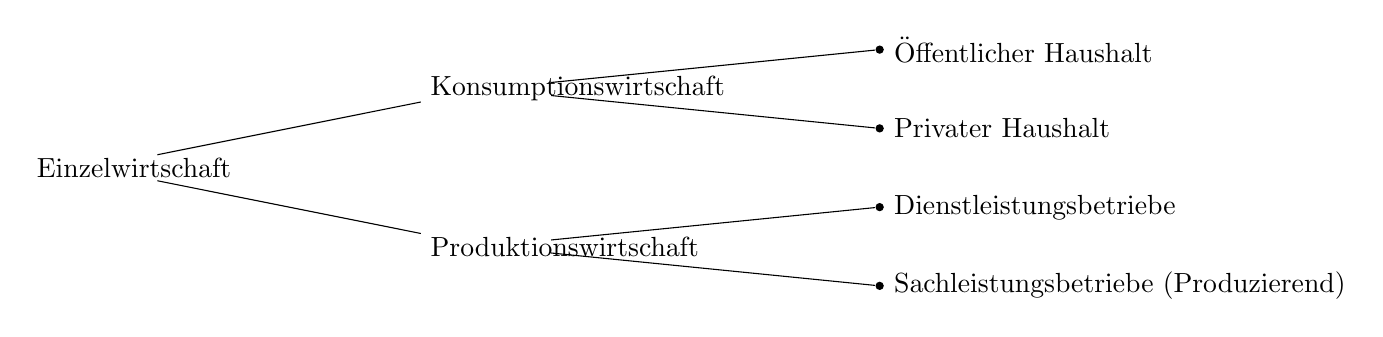
\begin{tikzpicture}[grow=right, sloped]
\node[bag] {Einzelwirtschaft}
    child {
        node[bag] {Produktionswirtschaft}        
            child {
                node[end, label=right:
                    {Sachleistungsbetriebe (Produzierend)}] {}
                edge from parent
                node[above] {}
                node[below]  {}
            }
            child {
                node[end, label=right:
                    {Dienstleistungsbetriebe}] {}
                edge from parent
                node[above] {}
                node[below]  {}
            }
            edge from parent 
            node[above] {}
            node[below]  {}
    }
    child {
        node[bag] {Konsumptionswirtschaft}        
        child {
                node[end, label=right:
                    {Privater Haushalt}] {}
                edge from parent
                node[above] {}
                node[below]  {}
            }
            child {
                node[end, label=right:
                    {Öffentlicher Haushalt}] {}
                edge from parent
                node[above] {}
                node[below]  {}
            }
        edge from parent         
            node[above] {}
            node[below]  {}
    };
\end{tikzpicture}
